\section{Introduction}
\label{sec:intro}
Bluesky replaces a single platform moderator with \emph{labels}~\cite{Bluesky_2023,Kleppmann_2024}. A labeler is an account that signs short values such as \texttt{spam} or \texttt{ai-imagery} and attaches them to posts or accounts~\cite{ATProto_labels}. Every client applies Bluesky's own labeler, and a signed-in user may subscribe to up to twenty more and decide, per label, whether to hide, warn or ignore. This realises the long-standing idea of moderation \emph{middleware}~\cite{Hogg_2024}, but it also fragments what people see. An author cannot tell which labels follow their account, a reader cannot tell what other readers are shown, and researchers have so far studied either the network's infrastructure~\cite{Balduf_2024} or Bluesky's own labeler~\cite{Singh_2026}, which explicitly leaves third-party labelers to future work.

LabelLens makes this fragmentation visible for one item at a time. Given a post link or a handle, it (i)~runs a \emph{census}, asking every labeler in a network-wide directory what it says about the post, its author and the author's profile, and (ii)~shows the item through \emph{lenses}, that is, subscription sets evaluated with the moderation code of the official client library. A companion \emph{Network} page summarises a measurement of all labelers. The demonstration offers three things: a tool anyone can run from a link, a census method that copes with a network where most services are unreachable from a browser, and measured evidence of how far the stacks diverge.

\begin{figure*}[t]
  \centering
  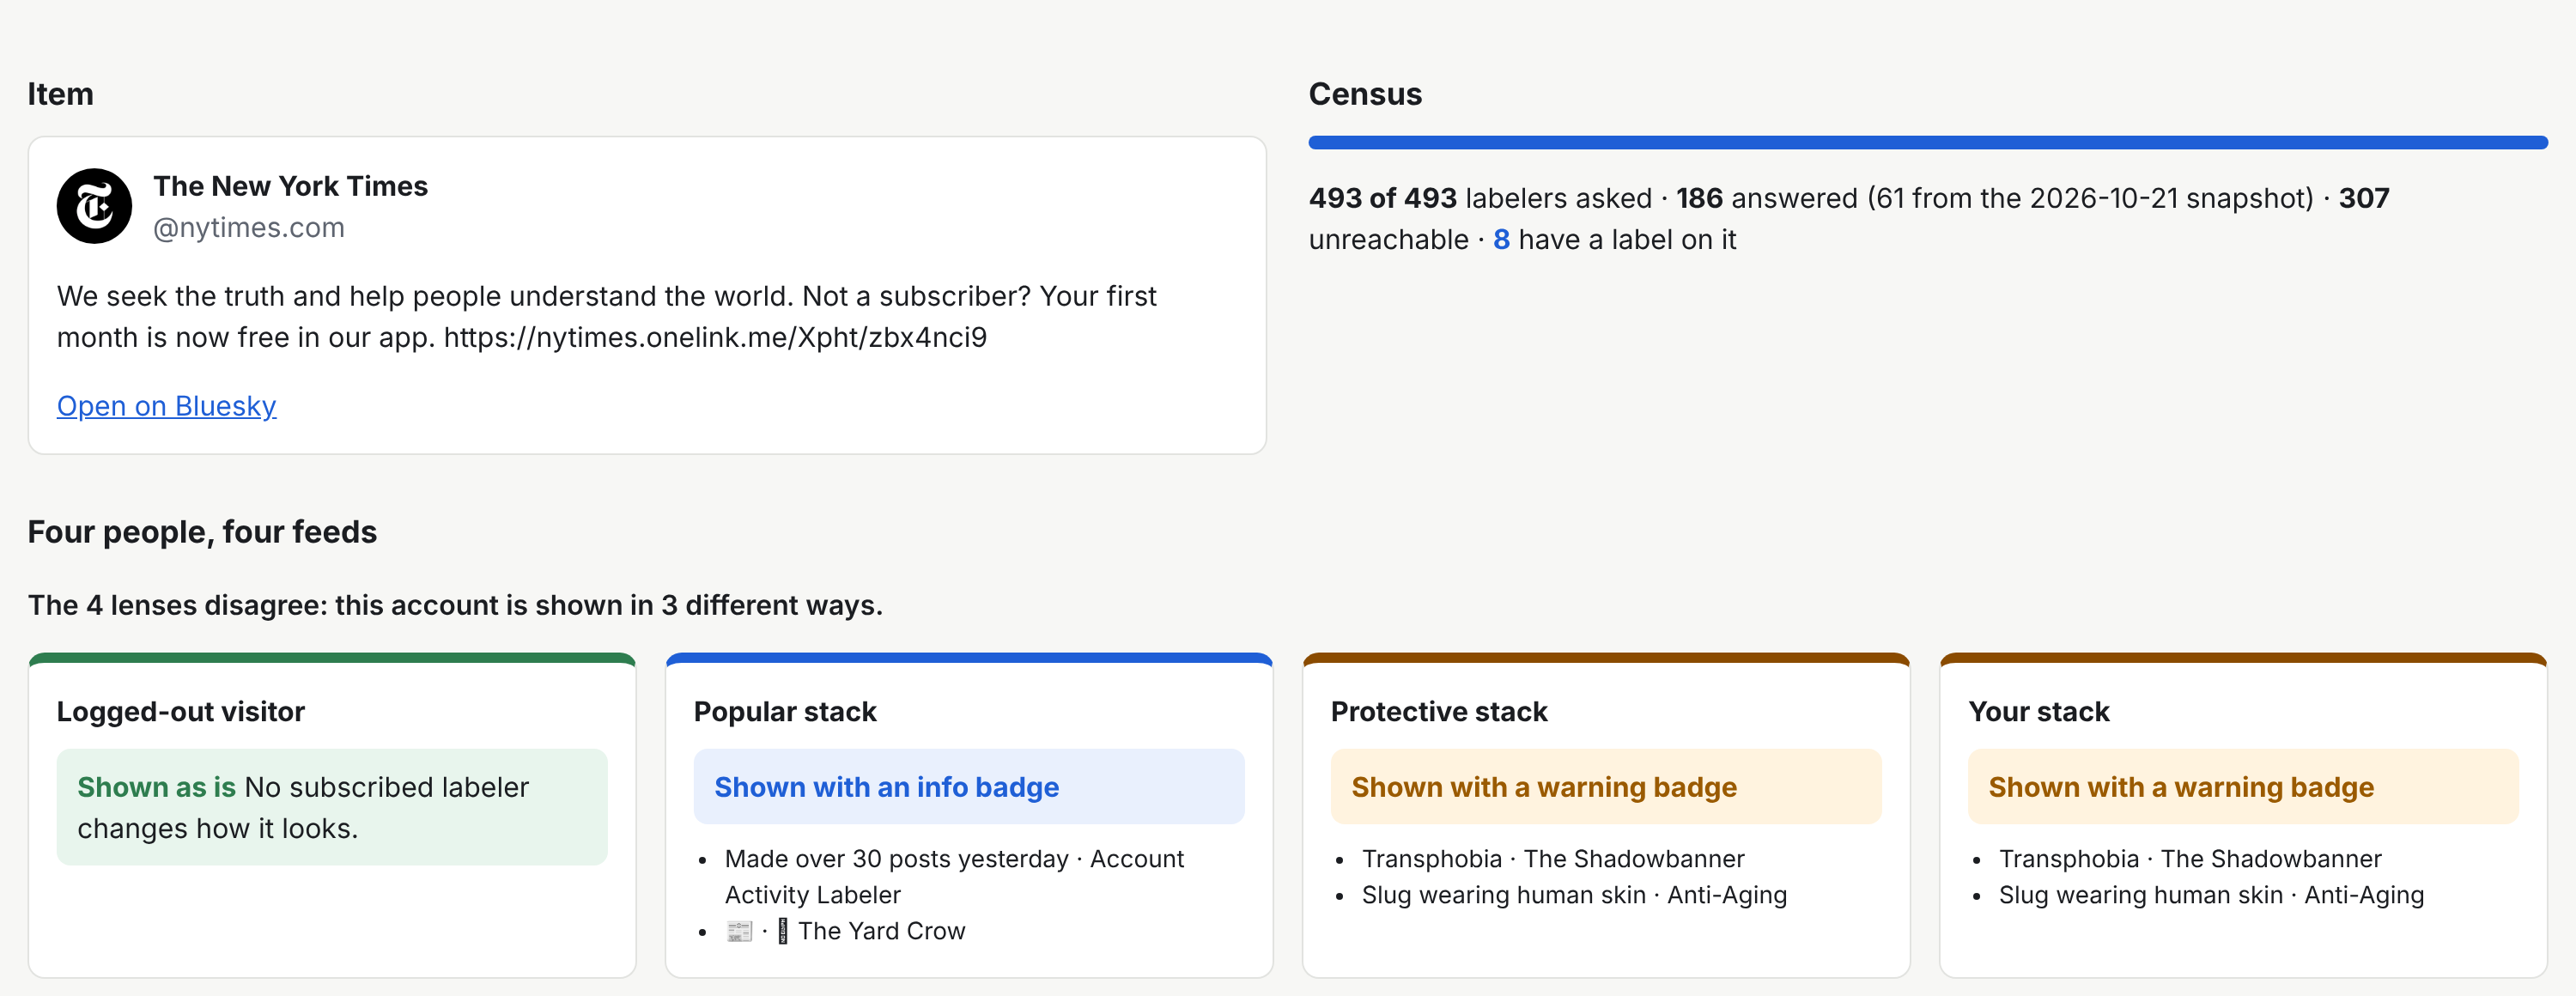
\includegraphics[width=\textwidth]{figures/ui_inspect.png}
  \caption{Inspecting a news organisation's account (\figDate): \figLabelers labelers label it, and the four lenses show it in \figOutcomes different ways. In this run \figAnswered services answered (\figLive live from the browser, \figSnapshot from the snapshot), against \labAnswering endpoints that answered our server-side probe (Section~\ref{sec:eval}). Labels are the labelers' own claims.}
  \label{fig:ui}
  \Description{Screenshot of the LabelLens Inspect page with the item, census progress, four lens cards and the per-labeler list.}
\end{figure*}
